\documentclass[10pt]{article}
\usepackage[a4paper,margin=2cm]{geometry}
\usepackage{amsmath,amssymb,amsthm,graphicx,hyperref}
\newtheorem{theorem}{Theorem}\newtheorem{proposition}[theorem]{Proposition}\newtheorem{lemma}[theorem]{Lemma}
\theoremstyle{definition}\newtheorem{definition}[theorem]{Definition}\newtheorem{remark}[theorem]{Remark}
\newcommand{\ip}[2]{\langle #1,#2\rangle}
\title{Circles as mirrors: the circle kei, and where two mirrors agree}
\author{Notes for Carlo Perassi --- companion to the reply Short}
\date{31 October 2026}
\begin{document}\maketitle
\begin{abstract}
We look at the operation ``reflect circle $D$ in circle $C$'' as a binary operation $C\star D$ on circle space $\mathbb P^3$.
It satisfies the axioms of a \emph{kei} (involutory quandle). It is closed on non-degenerate circles, isometric, and neither commutative nor associative.
For two mirrors $K,L$ we prove that the points where they \emph{agree} ($K\star P=L\star P$) are the two crossings together with the two limiting points. That makes four points over $\mathbb C$, of which exactly two are real.
So the pair Inigo Quilez calls ``hidden'' is half of a single object, and its visible partner is where the two mirrors agree.
Every numerical claim was checked in \texttt{alt\_verify.py} (log: \texttt{alt\_verify\_log.txt}).
\end{abstract}

\section{Circle space}
A generalised circle $a(x^2+y^2)+bx+cy+d=0$ is a point $[a:b:c:d]\in\mathbb P^3$; we allow complex entries.
Let
\[\ip XY = X^{\!\top}GY,\qquad G=\begin{pmatrix}0&0&0&-2\\0&1&0&0\\0&0&1&0\\-2&0&0&0\end{pmatrix},\qquad Q(X)=\ip XX=b^2+c^2-4ad .\]
$G$ has signature $(3,1)$.
For a real circle with centre $(x_0,y_0)$ and radius $r$ we have $X=[1:-2x_0:-2y_0:x_0^2+y_0^2-r^2]$ and $Q=4r^2$.
Lines have $a=0$ and $Q>0$. Points (circles of radius $0$) have $Q=0$. Real ``imaginary circles'' (radius$^2<0$) have $Q<0$.
Two circles are orthogonal iff $\ip XY=0$, and a point $P$ lies on $C$ iff $\ip PC=0$.

\section{The operation}
\begin{definition} For $Q(C)\neq 0$ put
\[ C\star D \;=\; s_C(D) \;=\; D-\frac{2\ip DC}{Q(C)}\,C .\]
\end{definition}
For real $C$ this is inversion in $C$ (reflection if $C$ is a line), applied to the circle $D$.
Since $s_C$ is linear and homogeneous of degree $0$ in $C$, it is well defined on $\mathbb P^3$.
Let $\mathcal X=\{[C]\in\mathbb{CP}^3: Q(C)\neq0\}$ and let $\mathcal X_{\mathbb R}$ be its real points.

\begin{proposition}[Isometry and closure]\label{p:iso}
$s_C$ is the orthogonal reflection in the hyperplane $C^\perp$. Hence $\ip{s_CX}{s_CY}=\ip XY$ and $Q(s_CX)=Q(X)$.
In particular $\star$ is closed on $\mathcal X$ and on $\mathcal X_{\mathbb R}$, and it preserves the sign of $Q$ on real circles.
\end{proposition}
\begin{proof}
$s_C$ fixes $C^\perp$ pointwise and sends $C\mapsto -C$. In $\ip{s_CX}{s_CY}$ the two cross terms $\mp4\ip XC\ip YC/Q(C)$ cancel.
\end{proof}

\begin{theorem}[The circle kei]\label{t:kei}
For all $C,D,E\in\mathcal X$:
\[\text{(K1) } C\star C=C,\qquad\text{(K2) } C\star(C\star D)=D,\qquad\text{(K3) } C\star(D\star E)=(C\star D)\star(C\star E).\]
So $(\mathcal X,\star)$ is a kei (involutory quandle), and so is $(\mathcal X_{\mathbb R},\star)$.
\end{theorem}
\begin{proof}
(K1) $s_C(C)=C-2C=-C$, which is the same point of $\mathbb P^3$. The axiom holds projectively, not on vectors.
(K2) $s_C^2=\mathrm{id}$, as for any reflection.
(K3) For an isometry $g$ we have $g\,s_D\,g^{-1}=s_{gD}$, because $s_{gD}(X)=X-2\ip X{gD}gD/Q(gD)=g\,s_D(g^{-1}X)$. Taking $g=s_C$ gives $s_C s_D s_C=s_{C\star D}$. Applying both sides to $C\star E=s_CE$ gives (K3).
\end{proof}
Thus $C\mapsto s_C$ embeds $\mathcal X$ into the conjugation quandle of reflections in $O(4)$; this is the standard way symmetric spaces give involutory quandles.
The fixed set of $s_C$ on $\mathbb P^3$ is $\{[C]\}\cup\mathbb P(C^\perp)$, so $[C]$ is an isolated fixed point. Hence $\mathcal X_{\mathbb R}^{Q>0}$ also satisfies Loos's axioms for a symmetric space \cite{Loos67,Loos69}.
Keis go back to Takasaki \cite{Tak43}, quandles to Joyce \cite{Joy82}; see Stanovsk\'y \cite{Sta15} for the history, including Euclidean reflections as the model example.

\paragraph{Numbers (verified).}
The operation is not commutative and not associative.
Take $K$ the unit circle, $L:\,y=1.7$, and $M$ the circle with centre $(1.5,0.8)$ and radius $1$. Then:
\begin{itemize}
\item $K\star L$ is the circle with centre $(0,0.2941)$ and radius $0.2941=1/3.4$.
\item $L\star K$ is the circle with centre $(0,3.4)$ and radius $1$.
\item $(K\star L)\star M$ has centre $(0.0862,0.3232)$ and radius $0.0574$.
\item $K\star(L\star M)$ has centre $(0.1873,0.3246)$ and radius $0.1248$.
\end{itemize}
Over $4000$ random triples (real circles, lines, imaginary circles, complex vectors), the largest errors were:
\begin{itemize}
\item (K1) $3\cdot10^{-16}$, (K2) $4\cdot10^{-12}$, (K3) $1.5\cdot10^{-11}$;
\item $Q$-invariance $3\cdot10^{-11}$, $\ip{}{}$-invariance $1\cdot10^{-11}$.
\end{itemize}

\begin{figure}[h]\centering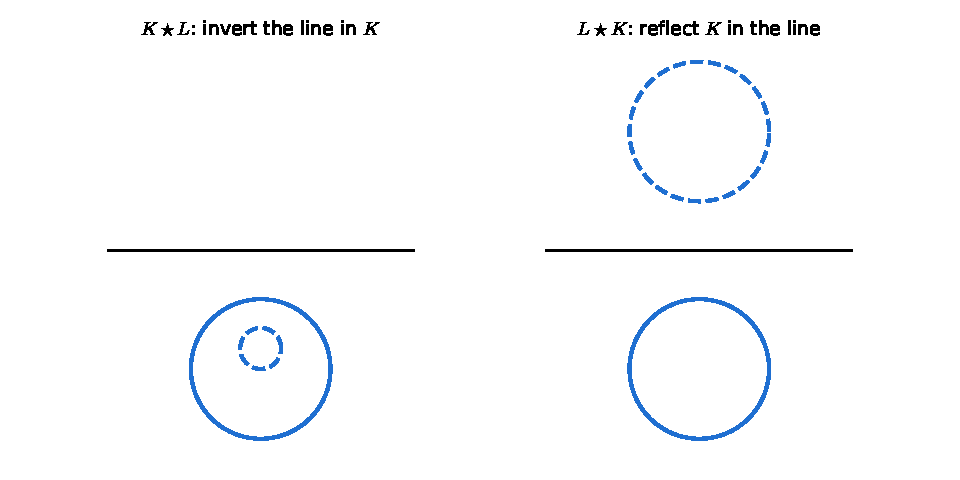
\includegraphics[width=.72\linewidth]{alt_figs/fig1_star.pdf}
\caption{Order matters. Left: the line $y=1.7$ inverted in the unit circle $K$ becomes a circle through the centre. Right: $K$ reflected in the line.}\end{figure}

\begin{remark}[Points cannot be mirrors]
If $Q(C)=0$ the formula is undefined. Clearing the denominator gives $Q(C)D-2\ip DC C\sim C$, so every $D$ goes to the point $C$.
This matches the limit: inverting a fixed circle in a mirror of radius $\varepsilon$ gives an image of radius $O(\varepsilon^2)$ that collapses onto the centre.
Numerically, radius $0.01$ gives an image of radius $7\cdot10^{-3}$, and radius $0.001$ gives $7\cdot10^{-5}$.
So points form a set that is \emph{acted on} ($s_C$ preserves $Q=0$) but does not act. This is the domain caveat.
\end{remark}

\begin{lemma}[What a mirror fixes]\label{l:fix}
$\mathrm{Fix}(s_C)=\{[C]\}\cup\{X:\ip XC=0\}$: the mirror itself, and every circle orthogonal to it.
The fixed \emph{points} ($Q=0$) are exactly the points lying on $C$.
\end{lemma}
\begin{proof}
$s_CX=\lambda X$ forces either $X\parallel C$ or $\ip XC=0$. For a point $P$, $\ip PC=0$ means $P\in C$.
\end{proof}

\section{Two mirrors: transport, common fixed circles, agreement}
\textbf{Transport.} Since $s_M$ is an isometry and preserves $Q=0$, it carries the point pair $K\cap L$ to $(M\star K)\cap(M\star L)$. It preserves the invariant
\[I=\frac{\ip KL^2}{Q(K)Q(L)},\]
so it sends a real pair to a real pair and a hidden pair to a hidden pair.
In the checks, $I$ was preserved for several values ($0.36$, $2.89$, $0.0156$, $4$), and the pair was transported with error $3.5\cdot10^{-15}$.

Fix real mirrors $K\neq L$ with $Q>0$, let $V=\mathrm{span}(K,L)$ and $U=V^\perp$. After normalising, the Gram matrix of $V$ is $\begin{pmatrix}1&g\\g&1\end{pmatrix}$ with $g^2=I$.
\begin{itemize}
\item If $I<1$ (the mirrors cut), $V$ has signature $(2,0)$, so $U$ has signature $(1,1)$.
\item If $I>1$ (disjoint or nested), $V$ has signature $(1,1)$, so $U$ has signature $(2,0)$.
\end{itemize}
The null lines of $U$ are the crossings $K\cap L$, real or hidden. The null lines of $V$ are the two \emph{limiting points} of the pencil $V$.

\begin{lemma}[Common fixed circles]
$\mathrm{Fix}(K)\cap\mathrm{Fix}(L)=\mathbb P(U)$ (for $K\not\perp L$).
If $I<1$ this is the Apollonian family around the two real crossings.
If $I>1$ it is the pencil of real circles through the two limiting points.
\end{lemma}
\begin{proof}
The first claim follows from Lemma \ref{l:fix}. A pencil contains real point-circles if and only if it has signature $(1,1)$. Its members then avoid those points. Signature $(2,0)$ means its members all pass through the null points of $U^\perp=V$.
Numerically, for $c=1.7$, $\max|\ip uP|=1.4\cdot10^{-15}$.
\end{proof}

\begin{theorem}[Where two mirrors agree --- ``always two points'']\label{t:agree}
Let
\[\mathrm{Agree}(K,L)=\{P:\;Q(P)=0,\ K\star P = L\star P\text{ in }\mathbb P^3\}.\]
Then:
\begin{enumerate}
\item $\mathrm{Agree}(K,L)$ is the union of the null points of $U$ (the crossings) and the null points of $V$ (the limiting points). Both mirrors fix the crossings, and both mirrors swap the two limiting points.
\item Over $\mathbb C$ this gives four points (for $I\neq 0,1$). Exactly two of them are real: the crossings if $I<1$, the limiting points if $I>1$. They merge into the tangency point if $I=1$.
\item $\mathrm{Agree}(K,L)\cap\hat{\mathbb C}=\mathrm{Fix}(s_L\circ s_K)$, the fixed points of a Möbius transformation. So in the real plane two distinct mirrors agree at exactly two points, or at one if they are tangent (count $\infty$ for lines).
\end{enumerate}
\end{theorem}
\begin{proof}
$s_KP\sim s_LP$ is equivalent to $s_Ls_KP\sim P$.
Write $P=u+v$ with $u\in U$ and $v\in V$. The map $s_Ls_K$ is the identity on $U$, and on $V$ it is a rotation (if $I<1$) or a boost (if $I>1$) by twice the angle between $K$ and $L$. Hence $P$ is an eigenvector exactly when $P\in U$ or $P$ lies on an eigenline of $s_Ls_K|_V$.
For $I\neq0,1$, the eigenlines of $s_Ls_K|_V$ are the null lines of $V$. Intersecting with $Q=0$ gives two points from $U$ and two from $V$.
Reality follows from the signatures above. On the limiting points $v_\pm$, $s_K$ and $s_L$ each act as the reflection of the hyperbolic plane $V$ in a non-null line, so they swap the two null lines.
For (3), the orientation-preserving composite $s_Ls_K$ acts on $\hat{\mathbb C}$ as a Möbius map $z\mapsto(\alpha z+\beta)/(\gamma z+\delta)$. Its fixed points solve a quadratic.
\end{proof}

\noindent\textbf{Our configuration.} Take $K=\{|z|=1\}$ and $L=\{y=c\}$. Then $s_K(z)=1/\bar z$ and $s_L(z)=\bar z+2ic$, so $s_Ls_K(z)=1/z+2ic$. The fixed points solve
\[z^2-2icz-1=0,\qquad z=ic\pm\sqrt{1-c^2}.\]
\begin{itemize}
\item $c=0.6$: $z=\pm0.8+0.6i$, the real crossings.
\item $c=1$: $z=i$, a double root (tangency).
\item $c=1.7$: $z=3.0748i$ and $z=0.3252i$, the limiting points $(0,c\pm\sqrt{c^2-1})$, whose heights multiply to $1$.
\end{itemize}
In the same case $c=1.7$, the hidden crossings are $(\pm1.3748i,\,1.7)$ in $\mathbb C^2$. These also satisfy $K\star P\sim L\star P$; they are the two non-real members of $\mathrm{Agree}$.
A brute-force search of the real plane found no other agreement points. Over $2000$ random real pairs ($981$ cutting, $1017$ disjoint or nested) there were $0$ mismatches with Theorem \ref{t:agree}.
Quilez's dots $(\pm\sqrt{c^2-1},c)$ are the limiting points rotated by $90^\circ$ about the foot $(0,c)$. This is the ``$i$'' of the hidden crossings made visible.

\begin{figure}[h]\centering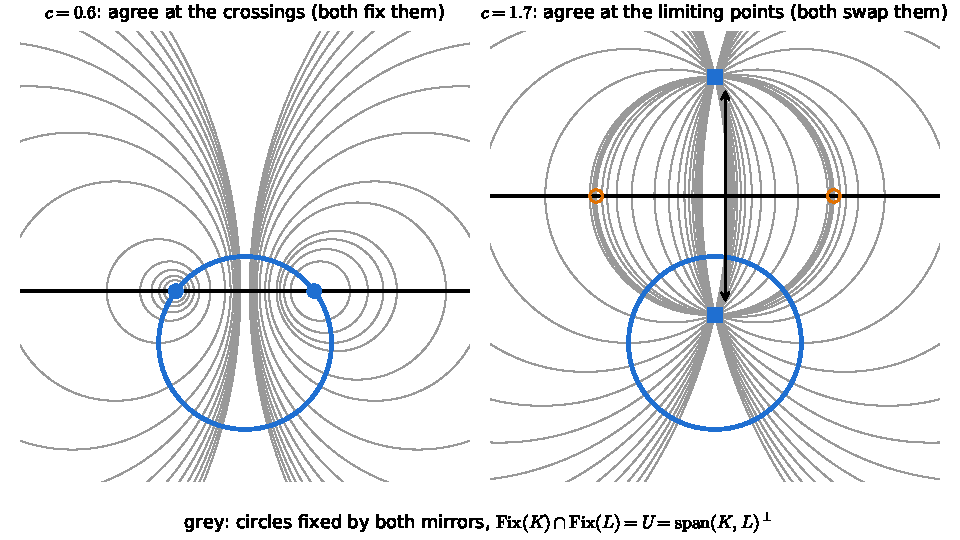
\includegraphics[width=.8\linewidth]{alt_figs/fig2_agree.pdf}
\caption{Agreement points (filled). Left: the line cuts, and the mirrors agree where they cross. Right: the line misses, the crossings are hidden (open circles mark Quilez's dots), and the mirrors agree at the limiting points, which both mirrors swap.}\end{figure}
\begin{figure}[h]\centering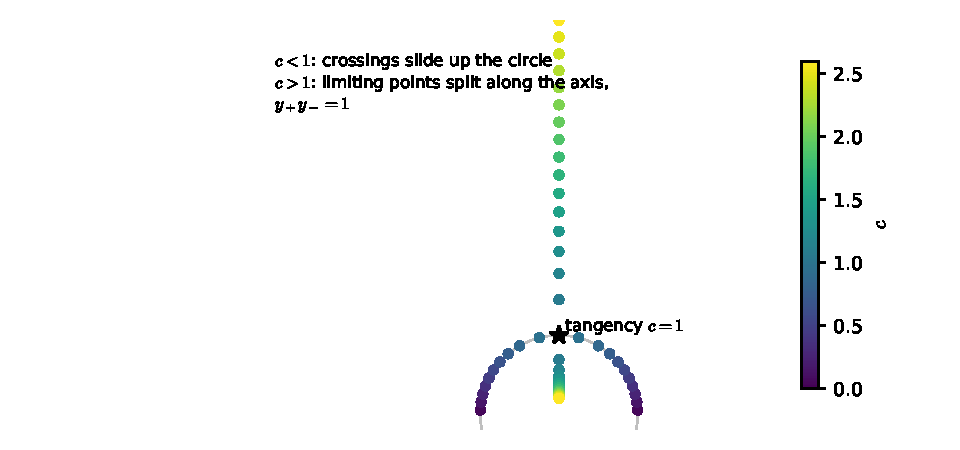
\includegraphics[width=.62\linewidth]{alt_figs/fig3_two.pdf}
\caption{The two real agreement points as the line rises. There are always two, except at tangency.}\end{figure}

\section{A note on $\mathbb P^3$ versus $\mathbb P^4$}
Everything above lives in Möbius circle space, the real $\mathbb P^3$ with a quadric of signature $(3,1)$. Its group is $PO(3,1)$, which is the Möbius group of the sphere, generated by inversions \cite{Sch79}.
Over $\mathbb C$, the quadric $\{Q=0\}\subset\mathbb{CP}^3$ is $\mathbb{CP}^1\times\mathbb{CP}^1$, and the point plane $\mathbb C^2$ sits inside it as an affine chart. This is where hidden crossings such as $(\pm1.3748i,1.7)$ live, so no extra dimension is needed.
\emph{Lie} sphere geometry instead puts \emph{oriented} circles in $\mathbb P^4$, on the Lie quadric of signature $(3,2)$, with group $O(3,2)/\pm I$ \cite{Cec08}. One can define the same reflection kei there. However, the agreement theorem does not need orientation or $\mathbb P^4$, so we stay in $\mathbb P^3$.

\begin{thebibliography}{9}\small
\bibitem{Tak43} M.~Takasaki, Abstractions of symmetric functions, \emph{Tohoku Math.\ J.} 49 (1943) 143--207 (in Japanese).
\bibitem{Joy82} D.~Joyce, A classifying invariant of knots, the knot quandle, \emph{J.\ Pure Appl.\ Algebra} 23 (1982) 37--65, doi:10.1016/0022-4049(82)90077-9.
\bibitem{Loos67} O.~Loos, Reflexion spaces and homogeneous symmetric spaces, \emph{Bull.\ AMS} 73 (1967) 250--253.
\bibitem{Loos69} O.~Loos, \emph{Symmetric Spaces}, Benjamin, 1969.
\bibitem{Sta15} D.~Stanovsk\'y, The origins of involutory quandles, arXiv:1506.02389.
\bibitem{Sch79} H.~Schwerdtfeger, \emph{Geometry of Complex Numbers}, Dover, 1979.
\bibitem{Cec08} T.~E.~Cecil, \emph{Lie Sphere Geometry}, 2nd ed., Springer Universitext, 2008, doi:10.1007/978-0-387-74656-2.
\end{thebibliography}
\end{document}
